\documentclass[runningheads]{llncs}
% ORTAK PREAMBLE -- main.tex ve supplementary.tex ikisi de bunu \input eder.
% Paket/makro/renk degisiklikleri YALNIZCA burada yapilir; iki dosya birbirinden kaymaz.

\usepackage[T1]{fontenc}
\usepackage{graphicx}
\usepackage{booktabs}
\usepackage{multirow}
\usepackage{amsmath,amssymb}
\usepackage{tikz}
\usepackage{pgfplots}
\pgfplotsset{compat=1.18}
\usetikzlibrary{arrows.meta,positioning,fit,backgrounds,shapes.geometric,decorations.pathreplacing}
\usepackage[hidelinks]{hyperref}
\usepackage{xr}

% Tool names, set once so a rename is a one-line change.
\newcommand{\Snape}{\textsc{snape}}
\newcommand{\Lcptools}{\textsc{Lcptools}}
\newcommand{\Lcpan}{\textsc{LCPan}}
\newcommand{\Gencore}{\textsc{GenCore}}
\newcommand{\Severus}{\textsc{Severus}}
\newcommand{\Minda}{\textsc{Minda}}

% Colours of the two-colored graph, used by every figure.
\definecolor{shared}{RGB}{110,110,110}
\definecolor{tumoronly}{RGB}{196,60,40}
\definecolor{normalonly}{RGB}{40,90,170}


% Ek malzeme AYRI bir PDF: supplementary.tex'in etiketleri (sup:*, tab:*) buradan
% \ref ile cagrilabilsin diye onun .aux'u okunuyor. Ikisini de iki kez derle.
\externaldocument{supplementary}
\begin{document}

\title{\Snape: Personalized tumor pangenomes from\\ somatic structural variants, without alignment}
\titlerunning{Personalized tumor pangenomes without alignment}

\author{Muti Kara \and Akmuhammet Ashyralyyev \and Can Alkan}
\authorrunning{M. Kara et al.}
\institute{Dept of Computer Engineering, Bilkent University, Ankara 06800, Turkey\\
\email{muti.kara@bilkent.edu.tr, akmuhammet@bilkent.edu.tr, calkan@cs.bilkent.edu.tr}}

\maketitle

\begin{abstract}
Somatic structural variant callers align every read set of a case to a reference before deciding which
reads are somatic, and take that decision one tumor at a time. \Snape{} reverses both. It partitions
one normal and $N$ tumor read sets by Locally Consistent Parsing into cores and counts them into a
single graph whose nodes carry an $(N{+}1)$-vector of per-sample counts: a core absent from the normal
is somatic \emph{by sequence}, and its tumor entries say which lines carry it. Each line's somatic
material is cut from its own reads as junction contigs and aligned independently, and the calls merge
into a \emph{personalized tumor pangenome} whose paths carry the lines supporting them. On the four
CASTLE pairs, the $N=1$ case, \Snape{} reaches F1 0.874 on HCC1954 and 0.754--0.865 on the rest,
against 0.810--0.903 for the published \Severus{} calls, in 39 minutes on 16 cores against 4 hours 7
minutes.
\smallskip

\noindent\textbf{Availability:} \url{https://github.com/Muti-Kara/snape}

\keywords{Locally consistent parsing \and somatic structural variation \and tumor pangenome \and
cancer genomics \and alignment-free methods}
\end{abstract}

\section{Introduction}\label{sec:intro}

Structural variants drive cancer genome evolution, and long reads resolve them where short reads
cannot~\cite{severus,savana}. The methods built on this share one design: align both the tumor and the
matched normal read set to a reference, read breakpoints off the alignments, cluster, and subtract
between the samples~\cite{severus,savana,nanomonsv}. Two properties follow from that order: aligning
both samples is the dominant cost, roughly 390 Gbp per pair here, and all of it is placed before the
first somatic decision; and the aligner assigns coordinates to sequence a somatic event has moved.

A third follows from the \emph{pairing}. A case is increasingly several tumors: regions of one mass, a
primary and its metastases, a longitudinal series. Run pairwise, the normal is aligned $N$ times, each
junction is discovered separately in every line carrying it, and whether two lines carry the
\emph{same} junction is settled afterwards by intersecting intervals — the step at which a shared
event placed differently becomes two.

The somatic question itself does not require a reference. It is a comparison between read sets: which
sequence do the tumor reads carry that the normal reads do not? That needs a way to recognize the same
locus in two different reads, and Locally Consistent Parsing (LCP) provides one. LCP partitions a
string into substrings called \emph{cores} under two guarantees~\cite{sv94a,sv94b}: \emph{partition
consistency}, that identical content is partitioned the same way wherever it occurs, and
\emph{labeling consistency}, that cores over the same sequence receive the same label. Applied
iteratively with Deterministic Coin Tossing~\cite{dct}, each level lengthens cores by
$c \approx 2.34$~\cite{lcpan,gencore}. Unlike sketching it subsamples nothing, so a somatic region
cannot fall between the samples and be missed.

\Snape{} takes the somatic decision before any alignment, for all $N$ lines at once
(Fig.~\ref{fig:overview}). One pass over the $N{+}1$ read sets builds a single core graph whose nodes
carry a vector of per-sample counts: a zero normal entry means somatic, and the tumor entries are the
\emph{support pattern}, exact because the labels are identical and before any coordinate exists. Each
line's contigs are then cut and aligned independently and the calls merge into a personalized tumor
pangenome, in which a junction shared by several lines is one object by construction rather than by
post-hoc interval matching, and an unlabelled read is assigned to a line by the private cores it
carries.

\begin{figure}[!t]
\centering
\resizebox{0.78\textwidth}{!}{%
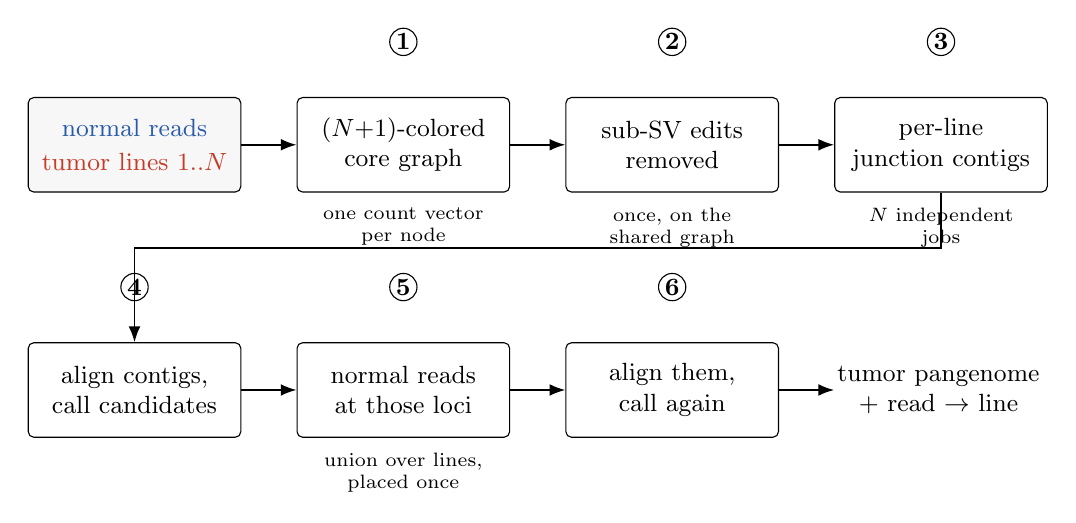
\begin{tikzpicture}[
  font=\small,
  box/.style={draw, rounded corners=2pt, align=center, minimum height=12mm, minimum width=27mm, inner sep=2pt},
  data/.style={align=center, inner sep=1pt},
  snum/.style={circle, draw, fill=white, inner sep=0.7pt, font=\small\bfseries},
  ar/.style={-{Latex[length=2mm]}, semithick},
  note/.style={align=center, font=\scriptsize, inner sep=1pt}
]
% ---------- row 1
\node[box, fill=black!3] (inp) at (0,0)
  {\textcolor{normalonly}{normal reads}\\[1pt]\textcolor{tumoronly}{tumor lines $1..N$}};
\node[box, right=7mm of inp] (graph) {$(N{+}1)$-colored\\core graph};
\node[box, right=7mm of graph] (bub) {sub-SV edits\\removed};
\node[box, right=7mm of bub] (ctg) {per-line\\junction contigs};
\draw[ar] (inp) -- (graph);
\draw[ar] (graph) -- (bub);
\draw[ar] (bub) -- (ctg);
\node[snum] at ([yshift=7mm]graph.north) {1};
\node[snum] at ([yshift=7mm]bub.north) {2};
\node[snum] at ([yshift=7mm]ctg.north) {3};
\node[note, below=1.5mm of graph] {one count vector\\ per node};
\node[note, below=1.5mm of bub] {once, on the\\ shared graph};
\node[note, below=1.5mm of ctg] {$N$ independent\\ jobs};

% ---------- row 2
\node[box, below=19mm of inp] (aln1) {align contigs,\\call candidates};
\node[box, right=7mm of aln1] (pick) {normal reads\\at those loci};
\node[box, right=7mm of pick] (aln2) {align them,\\call again};
\node[data, right=7mm of aln2] (out) {tumor pangenome\\+ read $\to$ line};
\draw[ar] (aln1) -- (pick);
\draw[ar] (pick) -- (aln2);
\draw[ar] (aln2) -- (out);
\node[snum] at ([yshift=7mm]aln1.north) {4};
\node[snum] at ([yshift=7mm]pick.north) {5};
\node[snum] at ([yshift=7mm]aln2.north) {6};
\node[note, below=1.5mm of pick] {union over lines,\\ placed once};

% row 1 -> row 2
\draw[ar] (ctg.south) -- ++(0,-7mm) -| (aln1.north);
\end{tikzpicture}}
\caption{\textbf{Overview.} \textbf{(1)} The normal and all $N$ lines are parsed into cores and counted
into one graph; a zero normal count means somatic, and the tumor counts name the lines carrying it.
\textbf{(2)} Local edits are dropped once, on the shared graph. \textbf{(3--4)} Each line's components
are cut from its own reads and aligned independently. \textbf{(5)} The union of the normal reads at
those loci is aligned once and decides which calls are germline. \textbf{(6)} What survives is one
pangenome whose paths carry their support patterns.}
\label{fig:overview}
\end{figure}

\section{Methods}\label{sec:methods}

\subsection{The multi-colored core graph}\label{sec:graph}

\Snape{} parses every read with \Lcptools~\cite{lcpan} at level $\ell = 5$, a core being a median of
217 bp of raw read, and represents the read by its core labels. Two reads covering one locus emit the
same labels over it whichever sample they come from, so sequence is equated by label rather than by
alignment; labels are computed over homopolymer-compressed bytes, to survive the errors the data
carries (Section~\ref{sup:cores}).

With $\mathcal{R}_0$ the normal read set and $\mathcal{R}_1,\dots,\mathcal{R}_N$ the tumor lines, let
$\mathbf{c}(x) = (c_0(x),\dots,c_N(x))$ count the retained cores carrying label $x$ in each sample.
The node set is
\begin{equation}\label{eq:nodes}
V = \{\,x : \max_i c_i(x) \geq \theta \,\},\qquad \theta = 3,
\end{equation}
a label seen fewer than $\theta$ times in every sample being read error. Color is not stored but read
off $\mathbf{c}$: $x$ is \emph{somatic} when $c_0(x) = 0$, and its \emph{support pattern} is
\begin{equation}\label{eq:pattern}
S(x) = \{\, i \in \{1,\dots,N\} : c_i(x) > 0 \,\},
\end{equation}
the set of lines carrying it — truncal when $S(x)$ is every line, private when it is one. The pairwise
design has no equivalent of \eqref{eq:pattern}, recovering the same partition only by comparing
coordinates after $N$ alignments. Edges are the adjacencies consecutive cores traverse, each with its
own count vector, so the graph holds no coordinates and no sequence and is built in one streaming pass
(Section~\ref{sup:impl}).

The somatic set is exact under stated conditions, the exception being a repeat where two samples spell
one locus differently while carrying the same allele (Section~\ref{sup:prop}).

\subsection{From somatic cores to junction contigs}\label{sec:contigs}

Most somatic cores are not structural variants: a somatic SNV or a short indel produces them too. Both
form a \emph{bubble}, two arms diverging and reconverging with one somatic, which the labels cannot
tell apart. \Snape{} separates them on two quantities, since a balanced junction changes no length and
a substitution changes no order. With $s_S, s_G$ the arms' spans in bases and $m_S, m_G$ their
minimizer sequences, the somatic arm is a local edit when
\begin{equation}\label{eq:bubble}
|s_S - s_G| \leq \sigma
\quad\text{and}\quad
|m_S| - \mathrm{lcs}(m_S, m_G) \leq 20 ,
\end{equation}
with $\sigma = 50$ bp, the caller's own size floor (Section~\ref{sup:bubblerule}). The test is on
sequence, not samples, so it runs once on the shared graph.

What survives induces a subgraph whose connected components are one junction candidate each;
restricting it to the nodes whose pattern contains line $i$ gives that line's candidates. For a read
of line $i$ carrying such a component, \Snape{} cuts the span from 50 cores before the somatic run to
50 cores after it: the novel sequence with about 5 kb of germline anchor on either side. That cut
needs no assembly, because consecutive cores of one read overlap in that read's own bytes
(Section~\ref{sup:contigrule}). Cutting, alignment and calling are therefore $N$ independent jobs over
one shared graph, and per line the aligner receives 1.76--6.20 Gbp against the 185--202 Gbp it was cut
from, a reduction of 32--105$\times$.

\subsection{Calling, the germline question, and the pangenome}\label{sec:call}

Contigs are aligned with \texttt{minimap2}~\cite{minimap2} and each junction is read off as a pair of
reference sides with the direction each leaves the reference in, which is the whole type vocabulary
and needs no typing step. Junctions agreeing on both sides to within 50 bp are one call, reported at
five supporting contigs (Section~\ref{sup:callrule}).

\Snape{} then reads the normal alignments at each call's locus and drops the call when the same event
is present there. Aligning the whole normal would restore the cost the method exists to avoid, $N$
times over, so the normal reads are chosen in core space: a call's contig anchors are sequence the
normal also carries, so \Snape{} streams the normal once and emits every read sharing at least five
anchor labels — 1.2--2.6\% of the sample, costing 0.004 of precision and no recall
(Section~\ref{sup:pick}) — and the union over lines is aligned once.

What survives is one \emph{personalized tumor pangenome}: the donor's genome plus every somatic
junction any line carries as an alternative path, each labelled with the support pattern
\eqref{eq:pattern} of its cores. Two lines carrying one junction contribute one path, because their
cores carry one label and not because two intervals overlapped, and a read is assigned to a line by
those same labels (Section~\ref{sup:assign}).

\section{Results}\label{sec:results}

We evaluated \Snape{} on four PacBio Revio tumor/normal pairs from the CASTLE panel, the $N = 1$ case,
on one 16-core workstation (Section~\ref{sup:data}). Accuracy is measured with \Minda~\cite{minda} at
the settings the panel reports against, applied unchanged to the published \Severus{} calls and to
ours. The graph has $7.0 \times 10^{7}$ nodes per pair, 0.54--1.48\% of them tumor-only: somatic
material inspectable without a reference (Section~\ref{sup:graph}).

\begin{figure}[!t]
\centering
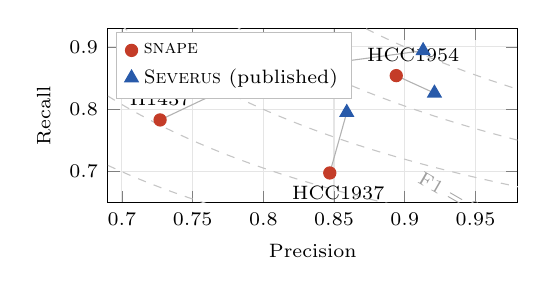
\begin{tikzpicture}
\begin{axis}[
  width=0.56\textwidth, height=3.8cm,
  xlabel={Precision}, ylabel={Recall},
  xmin=0.69, xmax=0.98, ymin=0.65, ymax=0.93,
  grid=major, grid style={draw=black!10},
  tick label style={font=\scriptsize}, label style={font=\scriptsize},
  legend style={font=\scriptsize, at={(0.02,0.98)}, anchor=north west, draw=black!25},
  legend cell align=left
]
% iso-F1 contours: R = F1 P / (2P - F1)
\foreach \f in {0.70,0.75,0.80,0.85,0.90}{
  \addplot[domain=0.69:0.98, samples=90, gray!45, dashed, thin, forget plot] {\f*x/(2*x-\f)};
}
% each pair's two points joined, so the comparison is read per sample
\addplot[gray!60, thin, forget plot] coordinates {(0.894,0.854) (0.921,0.826)};
\addplot[gray!60, thin, forget plot] coordinates {(0.854,0.876) (0.913,0.894)};
\addplot[gray!60, thin, forget plot] coordinates {(0.847,0.698) (0.859,0.795)};
\addplot[gray!60, thin, forget plot] coordinates {(0.727,0.783) (0.782,0.842)};
\addplot[only marks, mark=*, mark size=2.2pt, color=tumoronly] coordinates {
  (0.894,0.854) (0.854,0.876) (0.847,0.698) (0.727,0.783)};
\addlegendentry{\Snape}
\addplot[only marks, mark=triangle*, mark size=2.8pt, color=normalonly] coordinates {
  (0.921,0.826) (0.913,0.894) (0.859,0.795) (0.782,0.842)};
\addlegendentry{\Severus{} (published)}
\node[font=\scriptsize, anchor=south] at (axis cs:0.906,0.861) {HCC1954};
\node[font=\scriptsize, anchor=east] at (axis cs:0.848,0.876) {H2009};
\node[font=\scriptsize, anchor=north] at (axis cs:0.853,0.692) {HCC1937};
\node[font=\scriptsize, anchor=south] at (axis cs:0.727,0.790) {H1437};
\node[font=\scriptsize, gray!75, anchor=west, rotate=-30] at (axis cs:0.905,0.700) {F1 $=0.80$};
\end{axis}
\end{tikzpicture}
\caption{\textbf{Accuracy on the four CASTLE pairs ($N=1$).} Circles \Snape{}, triangles the published
\Severus{} calls, gray lines joining the two on one pair, dashed curves iso-F1. Numbers in
Table~\ref{tab:acc}, leave-one-caller-out in Table~\ref{tab:loo}.}
\label{fig:pr}
\end{figure}

\paragraph{Accuracy at $N = 1$.}
Fig.~\ref{fig:pr} plots precision and recall for the four pairs (Section~\ref{sup:acc}). On HCC1954
\Snape{} reaches F1 0.874 against \Severus{}'s 0.871, ahead on recall by 0.028 and behind on precision
by 0.027; on the other three it reaches 0.754--0.865 against 0.810--0.903. A \Severus{} vote is present
in 93.9--97.3\% of the truth records, so we also score on ensembles with each caller's own votes
removed: \Snape{} is then ahead on HCC1954 ($\Delta$F1 $+0.018$, McNemar $p = 4.8\times10^{-7}$),
behind on HCC1937 ($-0.027$), tied on the other two. By type it leads every compared caller on
breakends, 43\% of these truth sets, its deficit being indels below 200 bp
(Section~\ref{sup:bytype}). Removing the graph costs $0.259$ of precision for $0.019$ of recall
(Section~\ref{sup:ablation}).

\paragraph{Held-out data.}
At frozen parameters \Snape{} reaches F1 0.806 on HCC1395 and recall 0.726 on COLO829's 62 validated
events; against the exact truth of a simulated genome~\cite{insilicosv,badread} it recovers 527 of 600
adjacencies at 99.7\% precision and 1{,}358 of 1{,}602 at 98.6\% on a harder one
(Section~\ref{sup:sim}).

\paragraph{Cost.}
Fig.~\ref{fig:time} sets the pipeline against the alignment-first arm on HCC1954, sixteen cores pinned:
39 minutes against 4 hours 7 minutes, a factor of 6.3, at 1.6 times the peak memory
(Section~\ref{sup:arms}). Almost all of it is the aligner, which spends 3 hours 57 minutes placing
reads \Severus{} then processes in 9:47. That assumes the alignments are produced for this caller:
where a laboratory aligns both samples anyway, \Snape{} is four times \emph{slower} than 9:47 over
existing BAMs. The separation widens with $N$, since the graph pass and the normal alignment are paid
once (Section~\ref{sup:timing}).

\begin{figure}[!t]
\centering
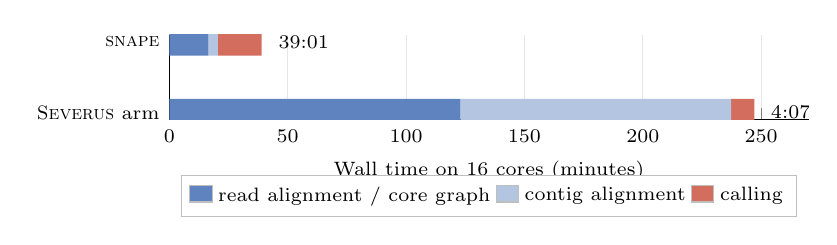
\begin{tikzpicture}
\begin{axis}[
  width=0.80\textwidth, height=2.6cm,
  xbar stacked,
  xmin=0, xmax=270,
  xlabel={Wall time on 16 cores (minutes)},
  ytick={0,1}, yticklabels={\Severus{} arm, \Snape},
  y=9mm,
  tick label style={font=\scriptsize}, label style={font=\scriptsize},
  legend style={font=\scriptsize, at={(0.5,-0.65)}, anchor=north, legend columns=3, draw=black!25},
  legend cell align=left,
  axis lines*=left,
  xmajorgrids, grid style={draw=black!10}
]
% row 0 = Severus arm: tumor align 122.95, normal align 114.38, caller 9.78  -> 247.11 (4:07:07)
% row 1 = snape:       graph/bubbles/junctions 16.48, contig align 4.00, call+pick+normal align 18.53 -> 39.01
\addplot[fill=normalonly!75, draw=none] coordinates {(122.95,0) (16.48,1)};
\addlegendentry{read alignment / core graph}
\addplot[fill=normalonly!35, draw=none] coordinates {(114.38,0) (4.00,1)};
\addlegendentry{contig alignment}
\addplot[fill=tumoronly!75, draw=none] coordinates {(9.78,0) (18.53,1)};
\addlegendentry{calling}
\node[font=\scriptsize, anchor=west] at (axis cs:250,0) {4:07:07};
\node[font=\scriptsize, anchor=west] at (axis cs:42,1) {39:01};
\end{axis}
\end{tikzpicture}
\caption{\textbf{What the two arms cost on HCC1954}, reads in to somatic VCF out, same 16 cores. The
alignment-first arm spends 2:02:57 and 1:54:23 placing the 196 and 195 Gbp read sets and 9:47 in
\Severus{}; \Snape{} spends 16:29 on the graph, 4:00 on 2.04 Gbp of contigs and 18:32 on calling plus
the normal reads the germline check needs (Table~\ref{tab:arms}).}
\label{fig:time}
\end{figure}

\paragraph{A twenty-line case.}
\textbf{[PLACEHOLDER --- not yet measured.]} The evaluation set is built and being sequenced in
silico: a germline genome carrying a real donor's 4,778,547 variants and a 39-node phylogeny whose 20
leaves carry 66,070 signature-placed somatic mutations, subclonal whole-genome duplication on two
branches, 20$\times$ HiFi per line (Section~\ref{sup:phylo}). Three quantities belong here: per-line
junction recall and precision; the Robinson--Foulds distance between the phylogeny \eqref{eq:pattern}
implies and the true one; and read-to-line assignment accuracy.

\section{Discussion}\label{sec:disc}

\Snape{} shows that a case's somatic decision can be taken in core space, before anything consults a
reference, leaving an alignment problem one to two orders of magnitude smaller. Two properties carry
it: partition consistency makes a locus produce the same core in every read set covering it, and
consecutive cores overlap, which makes a somatic region excisable from a single read. Generalizing the
color from a pair to an $(N{+}1)$-vector costs nothing and changes what the output is: not $N$ call
sets to reconcile, but one pangenome in which a junction shared by several lines is one object because
their cores share a label.

Three limitations bound this. The multi-line arm is specified but not measured, so every number above
is the $N = 1$ case. \Snape{} trails \Severus{} on indels below 200 bp, and the HCC1937 recall gap is
upstream of the caller, 66\% of its missed events having no contig at either breakpoint. And the two
properties used hold for $k$-mers and minimizers too, which we do not compare against, so the claim is
about the pipeline rather than the primitive.

\subsubsection{Data availability and contributions.}
Sequencing data are from BioProject PRJNA1086849 and truth sets from the CASTLE panel~\cite{castle};
\Snape{} is at \url{https://github.com/Muti-Kara/snape}. A.A. and C.A. conceived and supervised the
study; M.K. designed and implemented the method, ran the experiments and wrote the manuscript, which
all authors reviewed. The authors declare no competing interests.

\begin{thebibliography}{99}

\bibitem{severus} Keskus, A.G. et al. Severus detects somatic structural variation in cancer genomes
using long reads. Nat. Biotechnol. (2025).

\bibitem{savana} Elrick, H. et al. SAVANA: somatic structural variants and copy number from long
reads. Nat. Methods 22(7), 1436--1446 (2025).

\bibitem{nanomonsv} Shiraishi, Y. et al. Somatic complex structural variations from paired long-read
sequencing with nanomonsv. NAR 51(14), e74 (2023).

\bibitem{sv94a} Sahinalp, S.C., Vishkin, U. A parallel-algorithms method for string matching. CIAC '94,
LNCS 778, 22--32 (1994).

\bibitem{sv94b} Sahinalp, S.C., Vishkin, U. Symmetry breaking for suffix tree construction. STOC '94,
300--309 (1994).

\bibitem{dct} Cole, R., Vishkin, U. Deterministic coin tossing and accelerating cascades. STOC '86,
206--219 (1986).

\bibitem{lcpan} Ashyralyyev, A. et al. LCPan: variation graph construction using locally consistent
parsing. Genome Biol. 27 (2026).

\bibitem{gencore} Ashyralyyev, A. et al. GenCore: genomic distance estimation using LCP. bioRxiv (2026).

\bibitem{minda} Kolmogorov Lab. Minda. \url{https://github.com/KolmogorovLab/minda}

\bibitem{castle} CASTLE: Cancer Standards Long-read Evaluation. \url{https://github.com/CASTLE-Panel/castle}

\bibitem{insilicosv} Battistella, E. et al. insilicoSV: grammar-based structural variant simulation.
Bioinformatics 41(11), btaf594 (2025).

\bibitem{badread} Wick, R.R. Badread: simulation of error-prone long reads. JOSS 4(36), 1316 (2019).

\bibitem{minimap2} Li, H. Minimap2: pairwise alignment for nucleotide sequences. Bioinf. 34(18) (2018).

\bibitem{samtools} Danecek, P. et al. Twelve years of SAMtools. GigaScience 10(2) (2021).

\bibitem{murmur} Appleby, A. MurmurHash (2008).

\end{thebibliography}

\end{document}
